%!TEX program = xelatex
\documentclass{article}
\usepackage{amsthm,amsmath,amssymb}
\usepackage[UTF8]{ctex}
\usepackage[tc]{titlepic}
\usepackage{titlesec}
\usepackage{cite}
\usepackage{fancyhdr}
\usepackage{booktabs}
\usepackage{graphicx}
\usepackage{subfigure}
\usepackage{float} 
\usepackage{geometry}
\usepackage[section]{placeins}
\usepackage{makeidx}
\usepackage{mathrsfs}
\usepackage{color}
\usepackage{ulem}
\usepackage{enumitem}
\geometry{a4paper,scale=0.8}
\pagestyle{fancy}

\usepackage{hyperref}
\hypersetup{hypertex=true, colorlinks=true, linkcolor=blue, anchorcolor=blue, citecolor=blue}

\usepackage{listings}
\lstset{
    language=Python,
    basicstyle=\small\ttfamily,
    keywordstyle=\color{blue},
    commentstyle=\color{green},
    stringstyle=\color{red},
    showstringspaces=false,
    breaklines=true,
}

\lhead{第 2 次作业\\\today}
\chead{中国科学技术大学\\	DS4001 人工智能原理与技术}

\rhead{Homework 2\\ {\CTEXoptions[today=old]\today}}
\newcommand{\upcite}[1]{\textsuperscript{\cite{#1}}}

\titleformat*{\section}{\bfseries\Large}
\titleformat*{\subsection}{\bfseries\large}

\title{\bfseries 第二次作业(强化学习)}
\author{高茂航  \quad  PB22061161}

\begin{document}
\maketitle
\textcolor{red}{\textbf{本次作业需独立完成,不允许任何形式的抄袭行为,如被发现会有相应惩罚。在上方修改你的姓名学号,说明你同意本规定。}}
% \clearpage

\section*{问题1:热身(10分)}
\subsection*{a.计算(5分)}
    \begin{table}[h]
        \centering
        \begin{tabular}{|c|c|c|c|c|c|}
        \hline
        $i$ & $s=-2$ & $s=-1$ & $s=0$ & $s=1$ & $s=2$ \\
        \hline
        0 & 0 & 0 & 0 & 0 & 0 \\
        1 & 0&7.5 &-10 &20 & 0 \\
        2 & 0 & 2.5 & 5 & 16 & 0 \\
        \hline
        \end{tabular}
        \caption{Value Iteration for $i \in \{0, 1, 2\}$}
    \end{table}
\subsection*{b.计算(5分)}
$ (-1,a_2),(0,a_1),(1,a_1)$

\section*{问题2:Q-Learning(15分)}
\subsection*{a.回答问题(2分)}
状态值函数v(s)表示在状态s下的长期回报的期望,
而动作值函数q(s, a)表示在状态s下采取动作a后的长期回报的期望,
它们的计算基于整个MDP过程,而不依赖于任何特定的时间步。
\subsection*{b.计算(8分)}
$q^*(s, a) = (1-\alpha )q^*(s, a)+\alpha(r+\gamma q^*(s1, a1))$,

$t = 1$时$s=0$转移到$s=1$,此时$q^*(0, a1)=0,q^*(1, a)=0,\alpha=1$,$\therefore q^*(0, a1) = r_1=1$;

$t = 2$时$s=1$转移到$s=0$,此时$q^*(1, a1)=0,q^*(0, a)=1,\alpha=1$,$\therefore q^*(1, a1) = \alpha(r_2 +q^*(0, a))=3$;

$t = 3$时$s=0$转移到$s=1$,此时$q^*(0, a2)=0,q^*(1, a)=3,\alpha=1$,$\therefore q^*(0, a2) = \alpha(r_3+q^*(1, a))=2$。
\subsection*{c.回答问题(5分)}
在确定性环境中:

(1)Q-Learning算法基于贝尔曼方程,通过不断地更新Q值(在每个时间步都会选择当前最优的动作)来逼近贝尔曼方程的解,这个解就是最优的Q值。

(2)Q-Learning算法满足了所有状态-动作对的无限访问性条件,例如$\epsilon-greedy$策略。

(3)Q-Learning算法引入折扣因子$\gamma \in [0,1)$,
在学习率$\alpha \in (0,1]$时保证$\hat{Q}_n$在第k个遍历区间的误差小于$(\alpha\gamma+(1-\alpha))^k\Delta_0$。
\section*{问题3:Gobang Programming(55分)}
\subsection*{a.回答问题(2分)}
可行的,原因如下:

在$3\times3$的棋盘上,每个格子有三种可能的状态:空、玩家1的棋子、玩家2的棋子。因此,总的状态空间大小是$3^{(3*3)}=19683$,这是一个相对较小的状态空间,我们可以在合理的时间内遍历所有的状态。

对于每个状态,可能的动作是在空的格子上放一个棋子,因此动作空间的大小最多是9,这也是一个相对较小的动作空间。

由于状态空间和动作空间都相对较小,因此我们可以在合理的时间内计算出每个状态-动作对的Q值。

\subsection*{b.代码填空(33分)}
\begin{lstlisting}
class Gobang(UtilGobang):
    
    def get_next_state(self, action: Tuple[int, int, int], noise: Tuple[int, int, int]) -> np.array:

        # BEGIN_YOUR_CODE (our solution is 3 line of code, but don't worry if you deviate from this)
        black, x_black, y_black = action
        next_state = copy.deepcopy(self.board)
        next_state[x_black][y_black] = black
        # END_YOUR_CODE

        if noise is not None:
            white, x_white, y_white = noise
            next_state[x_white][y_white] = white
        return next_state

    def sample_noise(self) -> Union[Tuple[int, int, int], None]:

        if self.action_space:
            # BEGIN_YOUR_CODE (our solution is 2 line of code, but don't worry if you deviate from this)
            x, y = random.choice(self.action_space)
            self.action_space.remove((x, y))
            # END_YOUR_CODE
            return 2, x, y
        else:
            return None

    def get_connection_and_reward(self, action: Tuple[int, int, int],
                                  noise: Tuple[int, int, int]) -> Tuple[int, int, int, int, float]:

        # BEGIN_YOUR_CODE (our solution is 4 line of code, but don't worry if you deviate from this)
        black_1, white_1 = self.count_max_connections(self.board)
        next_state = self.get_next_state(action, noise)
        black_2, white_2 = self.count_max_connections(next_state)
        reward = (black_2 ** 2 - white_2 ** 2) - (black_1 ** 2 - white_1 ** 2)
        # END_YOUR_CODE

        return black_1, white_1, black_2, white_2, reward

    def sample_action_and_noise(self, eps: float) -> Tuple[Tuple[int, int, int], Tuple[int, int, int]]:

        # BEGIN_YOUR_CODE (our solution is 8 line of code, but don't worry if you deviate from this)
        if random.random() < eps or self.array_to_hashable(self.board) not in self.Q:
            x, y = random.choice(self.action_space)
        else:
            state = self.array_to_hashable(self.board)
            if self.Q[state]:
                _, x, y = max(self.Q[state], key=self.Q[state].get)
            else:
                x, y = random.choice(self.action_space)
        # END_YOUR_CODE
        return action, self.sample_noise()

    def q_learning_update(self, s0_: np.array, action: Tuple[int, int, int], s1_: np.array, reward: float,
                          alpha_0: float = 1):

        s0, s1 = self.array_to_hashable(s0_), self.array_to_hashable(s1_)
        self.s_a_visited[(s0, action)] = 1 if (s0, action) not in self.s_a_visited else \
            self.s_a_visited[(s0, action)] + 1
        alpha = alpha_0 / self.s_a_visited[(s0, action)]

        # BEGIN_YOUR_CODE (our solution is 18 line of code, but don't worry if you deviate from this)
        if s0 not in self.Q:
            self.Q[s0] = {}
        if action not in self.Q[s0]:
            self.Q[s0][action] = 0
        if s1 not in self.Q:
            self.Q[s1] = {}
        Q_x1_a1 = max(self.Q[s1].values(), default=0) if max(self.Q[s1].values(), default=0) > 0 else 0  
        self.Q[s0][action] = (1 - alpha) * self.Q[s0][action] + alpha * (reward + self.gamma * Q_x1_a1)
        # END_YOUR_CODE


\end{lstlisting}



\subsection*{c.结果复现(10分)}
\begin{figure}[H]
    \centering
    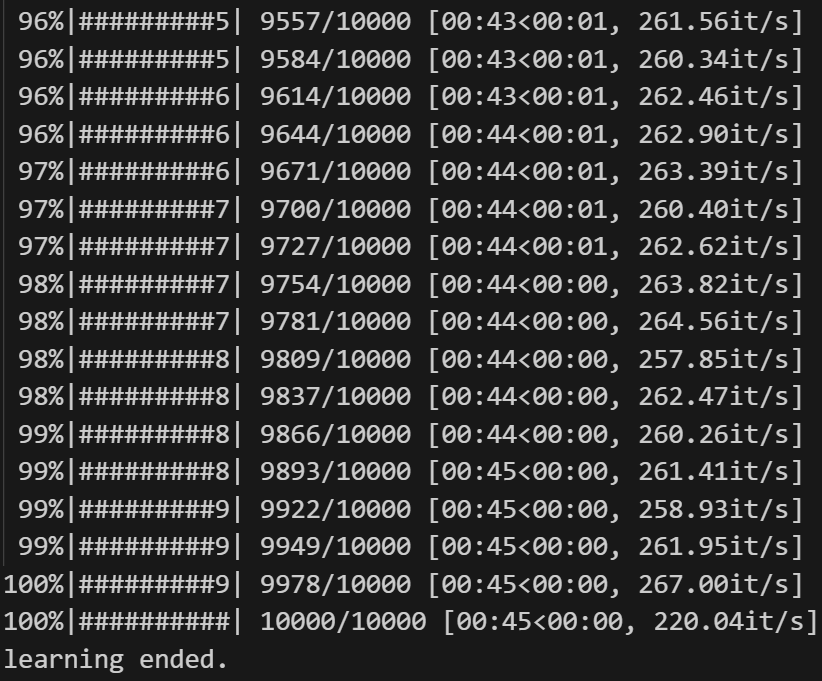
\includegraphics[width=14cm]{1.png}
\end{figure}
\begin{figure}[H]
    \centering
    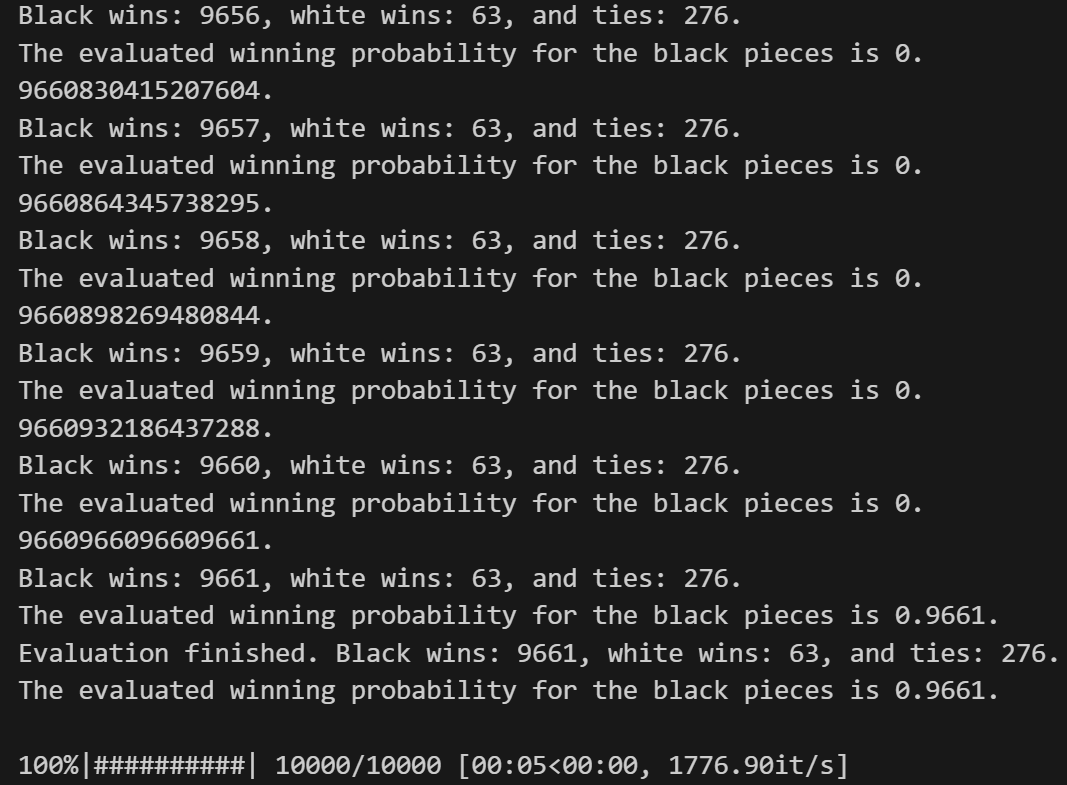
\includegraphics[width=14cm]{2.png}
\end{figure}

\subsection*{d.回答问题(10分)}

\begin{figure}[H]
    \centering
    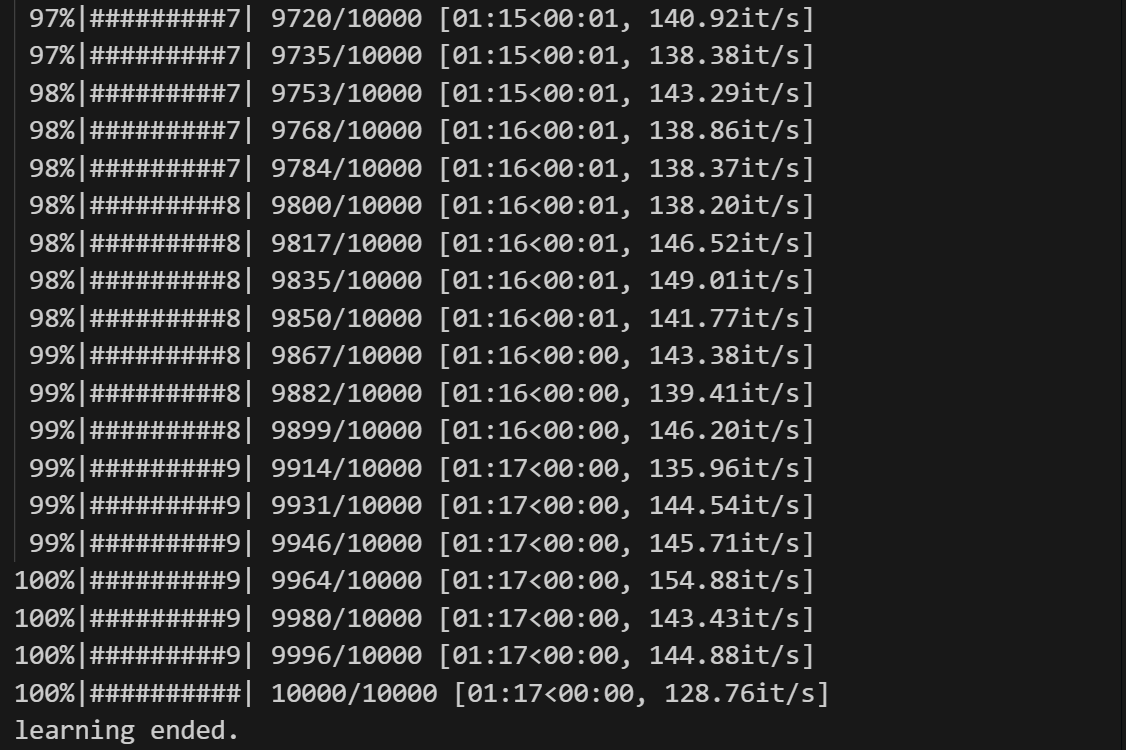
\includegraphics[width=14cm]{3.png}
\end{figure}
\begin{figure}[H]
    \centering
    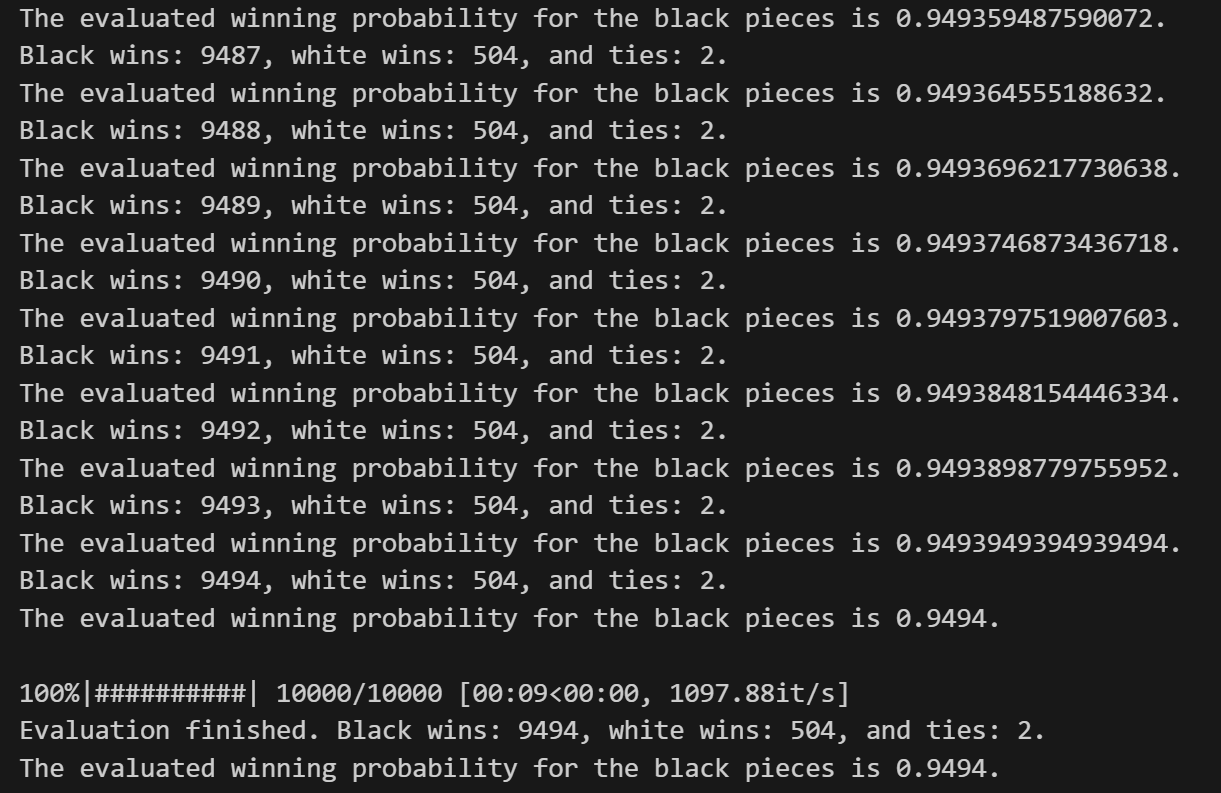
\includegraphics[width=14cm]{4.png}
\end{figure}
最终的胜率达到95\%左右,这个结果基本符合预期,因为通过合理地更新Q值使得agent能较好判断在每种状态下的最佳策略,但应该还可以继续微调以继续提高胜率。
\section*{问题4:Deeper Understanding(10分)}
\subsection*{a.回答问题(5分)}
确定性策略 $\mu$ 可以被表示为某个随机策略 $\pi$,其中 当 $a = \mu(s)$时$\pi(s, a) = 1$ ,否则 $\pi(s, a) = 0$,$\mathcal{T}_\mu$ 的定义如下:

\[
(\mathcal{T}_\mu v)(s) = r_{s,\mu(s)} + \gamma \sum_{s' \in S} p_{s,\mu(s),s'} v(s')
\]
\subsection*{b.回答问题(5分)}
对$\forall  v1, v2 \in \mathbb{R}^{|\mathcal{S}|}$
,我们有\begin{align*}
    \|\mathcal{T} v_1 - \mathcal{T} v_2\|_\infty &= \max_{s \in S} |(\mathcal{T} v_1)(s) - (\mathcal{T} v_2)(s)| \\
    &= \max_{s \in S} \left|\max_{a \in A} \left\{r_{s,a} + \gamma \sum_{s' \in S} p_{s,a,s'} v_1(s')\right\} - \max_{a \in A} \left\{r_{s,a} + \gamma \sum_{s' \in S} p_{s,a,s'} v_2(s')\right\}\right| \\
    &\leq \max_{s \in S} \max_{a \in A} \left|\gamma \sum_{s' \in S} p_{s,a,s'} (v_1(s') - v_2(s'))\right| \\
    &\leq \gamma \max_{s \in S} \max_{a \in A} \sum_{s' \in S} p_{s,a,s'} |v_1(s') - v_2(s')| \\
    &= \gamma \max_{s \in S} \max_{a \in A} \sum_{s' \in S} p_{s,a,s'} \|\mathcal{T} v_1 - \mathcal{T} v_2\|_\infty \\
    &= \gamma \|v_1 - v_2\|_\infty
\end{align*}


所以得证。


\section*{反馈(10分)}

\begin{itemize}
    \item 大概是两天时间,感觉比第一次的代码难度低一些,
    但在基础知识的学习理解上花了更多时间,特别是数学公式的推导感觉比较困难。
    
\end{itemize}

\end{document}